\appendix
\setcounter{equation}{0}
\setcounter{figure}{0}
\renewcommand{\theequation}{A.\arabic{equation}}
\renewcommand\thefigure{A.\arabic{figure}}

\section{Online appendix}
\label{sec:Appendix}

This is the Online Appendix for the paper:

\begin{center}
Rodríguez-Sánchez P, van Nes EH, Scheffer M. \textit{Neutral competition boosts chaos in food webs}.
\end{center}

\subsection{Chaos detection}
\label{subsec:ChaosDetection}
In the exploratory phase of this research three parallel approaches to chaos detection were followed: Lyapunov exponents estimation  \citep{Strogatz1994}, Gottwald - Melbourne \textit{0-1} test \citep{Gottwald2009} and visual inspection. Despite differences in the exact probabilities, the three of them led us to the same qualitative conclusions (see figure \ref{fig:AllContours}). We found the Gottwald - Melbourne test to be the fastest and most reliable of all.

\begin{figure}[H]
	\begin{center}
		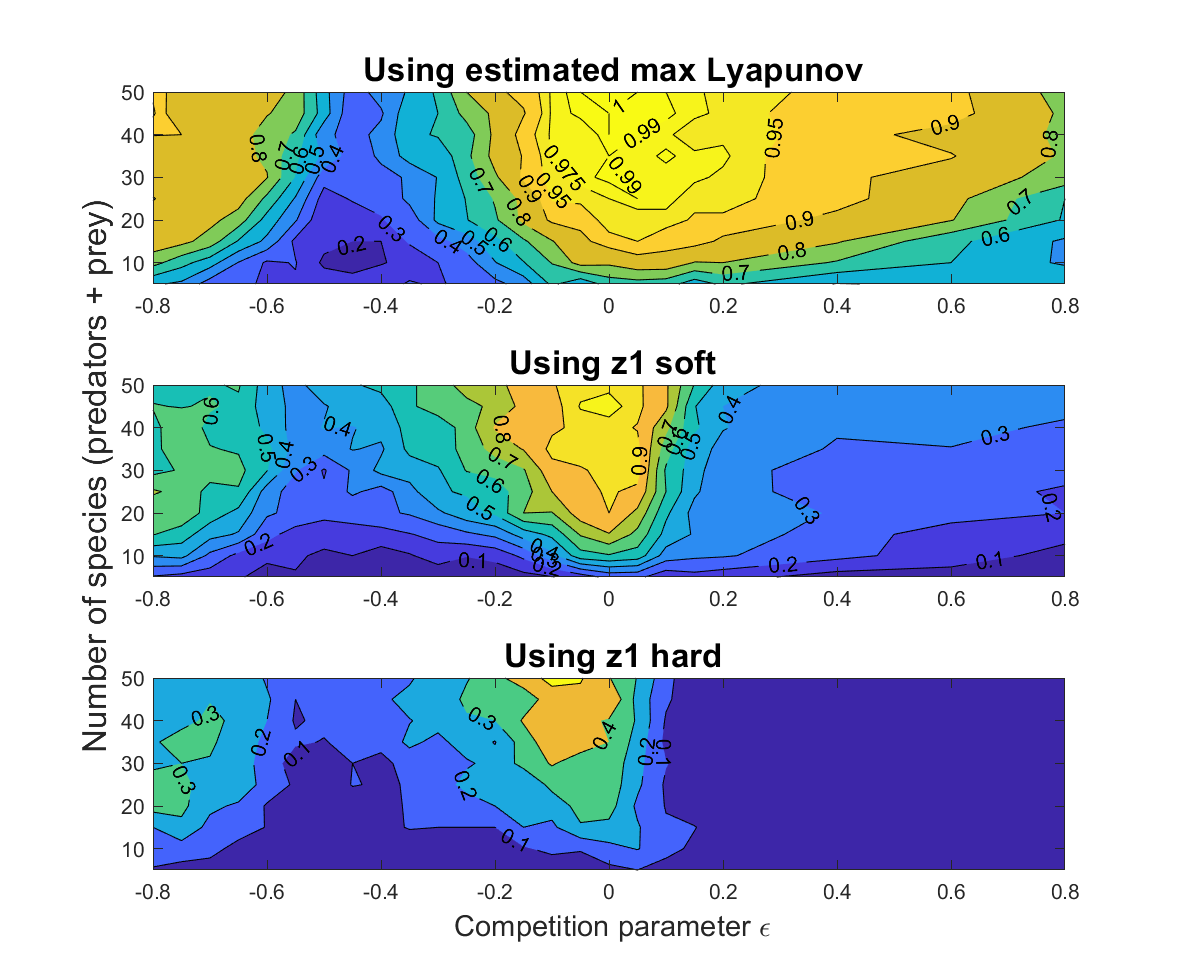
\includegraphics[width=1\columnwidth]{contours_all.png}
	\end{center}
	\caption{Performing the same analysis with different chaos detection algorithms we found different numerical results. The upper panel used the estimation of the maximum Lyapunov exponent as a test for chaoticity. The second and third used the z1 Gottwald - Melbourne test, with different degrees of tolerance. In particular, \textit{z1 soft} is more prone to classify complicated cycles as chaos, and \textit{z1 hard} is more likely to throw indecisive results. Even for the most conservative test (\textit{z1 hard}), the qualitative conclusions (that is, that chaos happens more frequently in the vicinity of neutral competition) still hold.}
	\label{fig:AllContours}
\end{figure}

\subsubsection{Melbourne-Gottwald 0-1 test in a nutshell}
\label{subsubsec:z1test}
The 0-1 test for chaos is designed for distinguishing between regular and chaotic dynamics in deterministic systems. It works directly with the observed time series, so a prior knowledge of the underlying dynamics is not required (as long as we know that they are deterministic).

This short section is more a motivation than a rigorous proof. A minimal, intuitive approach to the method will be outlined. For a detailed, complete explanation please refer to \citet{Gottwald2009}.

First, we have to use one of our time series of observations $\phi_k$ to build the functions:
%
\begin{eqnarray}
\label{eq:z1}
	\begin{cases}
	p_n(\theta) = \sum_{k=1}^n \phi_k cos(k \theta)
	\\
	q_n(\theta) = \sum_{k=1}^n \phi_k sin(k \theta)
	\end{cases}
\end{eqnarray}
%
Using Euler's formula both equations can be given a more compact form:
%
\begin{equation}
\label{eq:z1complex}
z_n(\theta) = p_n(\theta) + i q_n(\theta) = \sum_{k=1}^n \phi_k e^{i k \theta}
\end{equation}
%
In the complex plane, $e^{i k \theta}$ represents a unit vector pointing in the direction $k \theta$. So each observation in our time series can be understood as the size of a step, being $k \theta$ its direction (see table \ref{tab:Summands}).

\begin{table}[H]
\begin{center}
\begin{tabular}{|c|c|c|c|c|c|}
\hline
k & 0 & 1 & 2 & 3 & ...\\
\hline
$k \theta$ & 0 & $\frac{\pi}{6}$ & $\frac{2\pi}{6}$ & $\frac{\pi}{2}$ & ...\\
\hline
$e^{i k \theta}$ & 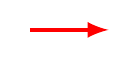
\begin{tikzpicture} \draw[->, ultra thick, red,  arrows={-latex}] (0,0) -- (1,0); \end{tikzpicture} & 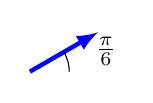
\begin{tikzpicture} \draw[->, ultra thick, blue,  arrows={-latex}]  (0,0) -- (0.866,0.5); \draw (0.5,0) arc (0:30:0.5) node[] at (15:1) {$\frac{\pi}{6}$}; \end{tikzpicture} & 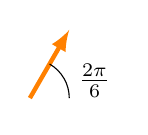
\begin{tikzpicture} \draw[->, ultra thick, orange,  arrows={-latex}]  (0,0) -- (0.5,0.866); \draw (0.5,0) arc (0:60:0.5) node[] at (15:0.85) {$\frac{2\pi}{6}$}; \end{tikzpicture} & 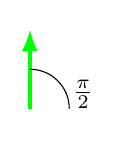
\begin{tikzpicture} \draw[->, ultra thick, green,  arrows={-latex}]  (0,0) -- (0,1); \draw (0.5,0) arc (0:90:0.5) node[] at (15:0.7){$\frac{\pi}{2}$}; \end{tikzpicture} & ... \\
\hline
$\phi_k$ & 2 & 1 & 0.5 & 0.25 & ...\\
\hline
$\phi_k e^{i k \theta}$ & 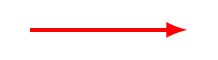
\begin{tikzpicture} \draw[->, ultra thick, red,  arrows={-latex}]  (0,0) -- (2,0); \end{tikzpicture} & 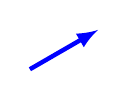
\begin{tikzpicture} \draw[->, ultra thick, blue,  arrows={-latex}]  (0,0) -- (0.866,0.5); \end{tikzpicture} & 
\begin{tikzpicture} \draw[->, ultra thick, orange,  arrows={-latex}]  (0,0) -- (0.25,0.433); \end{tikzpicture} & 
\begin{tikzpicture} \draw[->, ultra thick, green,  arrows={-latex}]  (0,0) -- (0,0.25); \end{tikzpicture} & ... \\
\hline
\end{tabular}
\end{center}
\caption{\label{tab:Summands} Example showing a step by step geometrical construction of the elements inside the summation operator in equation \eqref{eq:z1complex}. In this example we use a time series whose first elements are $\phi_j = \left\lbrace 2, 1, 0.5, 0.25, ...\right\rbrace$. The parameter $\theta$ has been set to $\frac{\pi}{6}$.}
\end{table}

Adding up the elements in table \ref{tab:Summands} as indicated by equation \eqref{eq:z1complex} can be interpreted geometrically as vector addition, i.e., performing one "step" after another (see figure \ref{fig:Sum}).

\begin{figure}[H]
\begin{center}
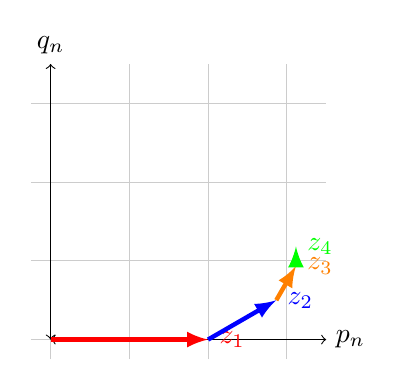
\begin{tikzpicture}
	% Grid
  	\draw[thin,gray!40] (-0.25,-0.25) grid (3.5,3.5);

  	% Axes
    \draw[<->] (0,0)--(3.5, 0) node[right]{$p_n$};
  	\draw[<->] (0,0)--(0, 3.5) node[above]{$q_n$};

	% Data
  	\draw[->, ultra thick, red,  arrows={-latex}]  (0,0) -- (2,0) node[right]{$z_1$};
  	\draw[->, ultra thick, blue,  arrows={-latex}]  (2,0) -- (2.866,0.5) node[right]{$z_2$};
  	\draw[->, ultra thick, orange,  arrows={-latex}]  (2.866,0.5) -- (3.116,0.933) node[right]{$z_3$};
  	\draw[->, ultra thick, green,  arrows={-latex}]  (3.116,0.933) -- (3.116,1.183) node[right]{$z_4$};

\end{tikzpicture}
\end{center}
\caption{\label{fig:Sum} Geometrical calculation of $z_1, z_2, z_3$ and  $z_4$ for $\phi_j = \left\lbrace 2, 1, 0.5, 0.25, ...\right\rbrace$ and $\theta = \frac{\pi}{6}$.}
\end{figure}

With this picture in mind, it is easy to understand the kind of paths that different types of time series will give rise to (see figure \ref{fig:z1Path}). Constant time series generate cyclic paths (polygons) or pseudocyclic paths (polygons that do not close after a first round). Periodic or pseudoperiodic time series generate periodic or pseudoperiodic paths (note that the summand in \eqref{eq:z1complex} becomes then the product of two periodic/pseudoperiodic functions). Random time series generate brownian-motion-like paths. Provided that our system is deterministic, the apparent stochasticity of our observed time series is a strong indicator of chaos.

\begin{figure}
	\begin{center}
		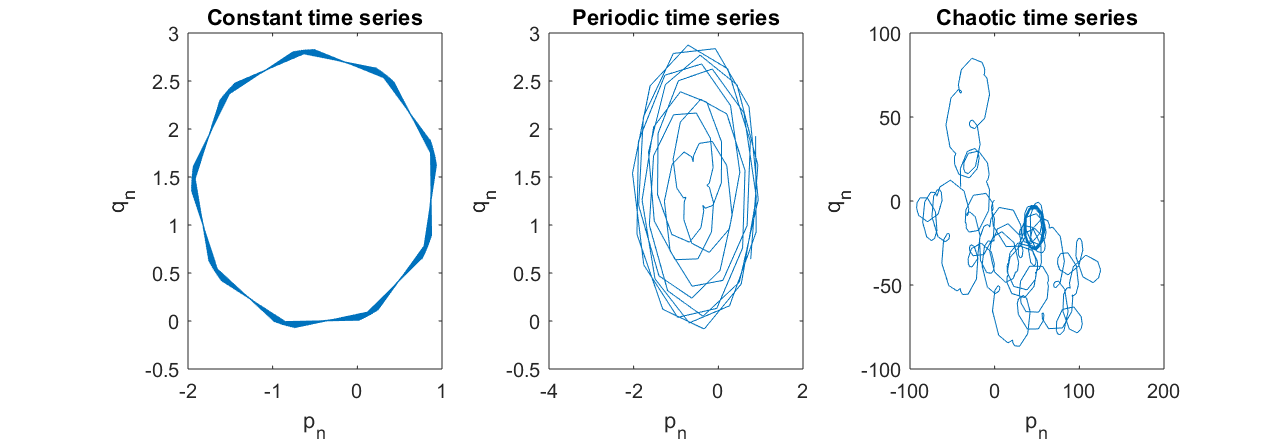
\includegraphics[width=1\columnwidth]{z1.png}
	\end{center}
	\caption{First and second panels show the paths generated by the z1 test when applied to constant and periodic time series. The third panel shows the case with a chaotic time series (notice the different scale). While in the first two cases the paths remain inside a bounded domain, in the chaotic case the path drifts away from the starting point in a brownian-motion-like fashion.}
	\label{fig:z1Path}
\end{figure}

The case of an underlying chaotic time series is the only one that generates a path that doesn't stay inside a bounded domain around the starting point. The z1 test uses the mean square displacement as a measure of this drift. The system is considered to be chaotic if the square displacement keeps growing for large times. If, on the contrary, it stays bounded, the test will consider the system not chaotic.


\subsection{Extra figures}
\label{subsec:ExtraFigures}

\subsubsection{Multispecies predator-prey network}
\label{subsubsec:MultispeciesPPNetwork}
\begin{figure}[H]
	\begin{center}
		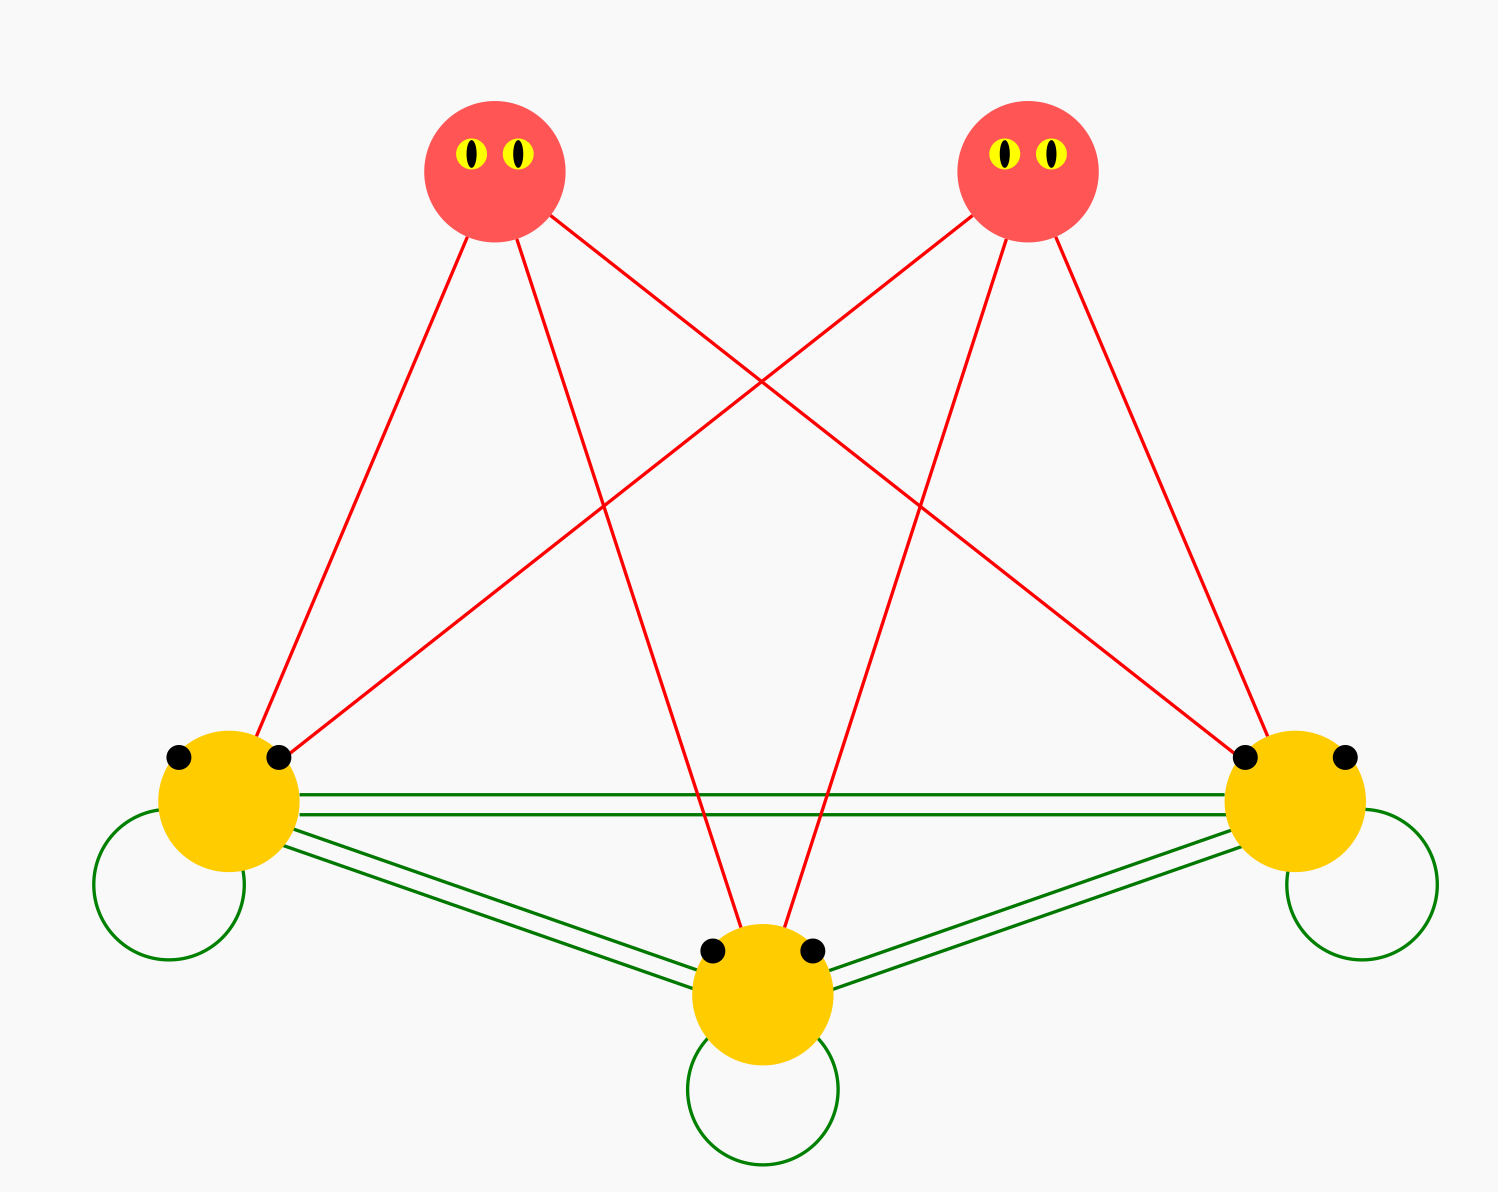
\includegraphics[width=0.5\columnwidth]{net.png}
	\end{center}
	\caption{Example with $2$ consumers and $3$ prey. Each one of the red links represents a predation interaction (coded in the matrix of predator preference coefficients, $ S $). Each green link represents a competition interaction (coded in the matrix of competition coefficients, $ A $). The closed green loops are related with carrying capacity (diagonal elements of $ A $) interpreted here as intra-species competition.}
	\label{fig:Network}
\end{figure}

\subsubsection{Probabilities grouped by number of species}
\label{subsubsec:AllProbabilities}
\begin{figure}[H]
	\begin{center}
		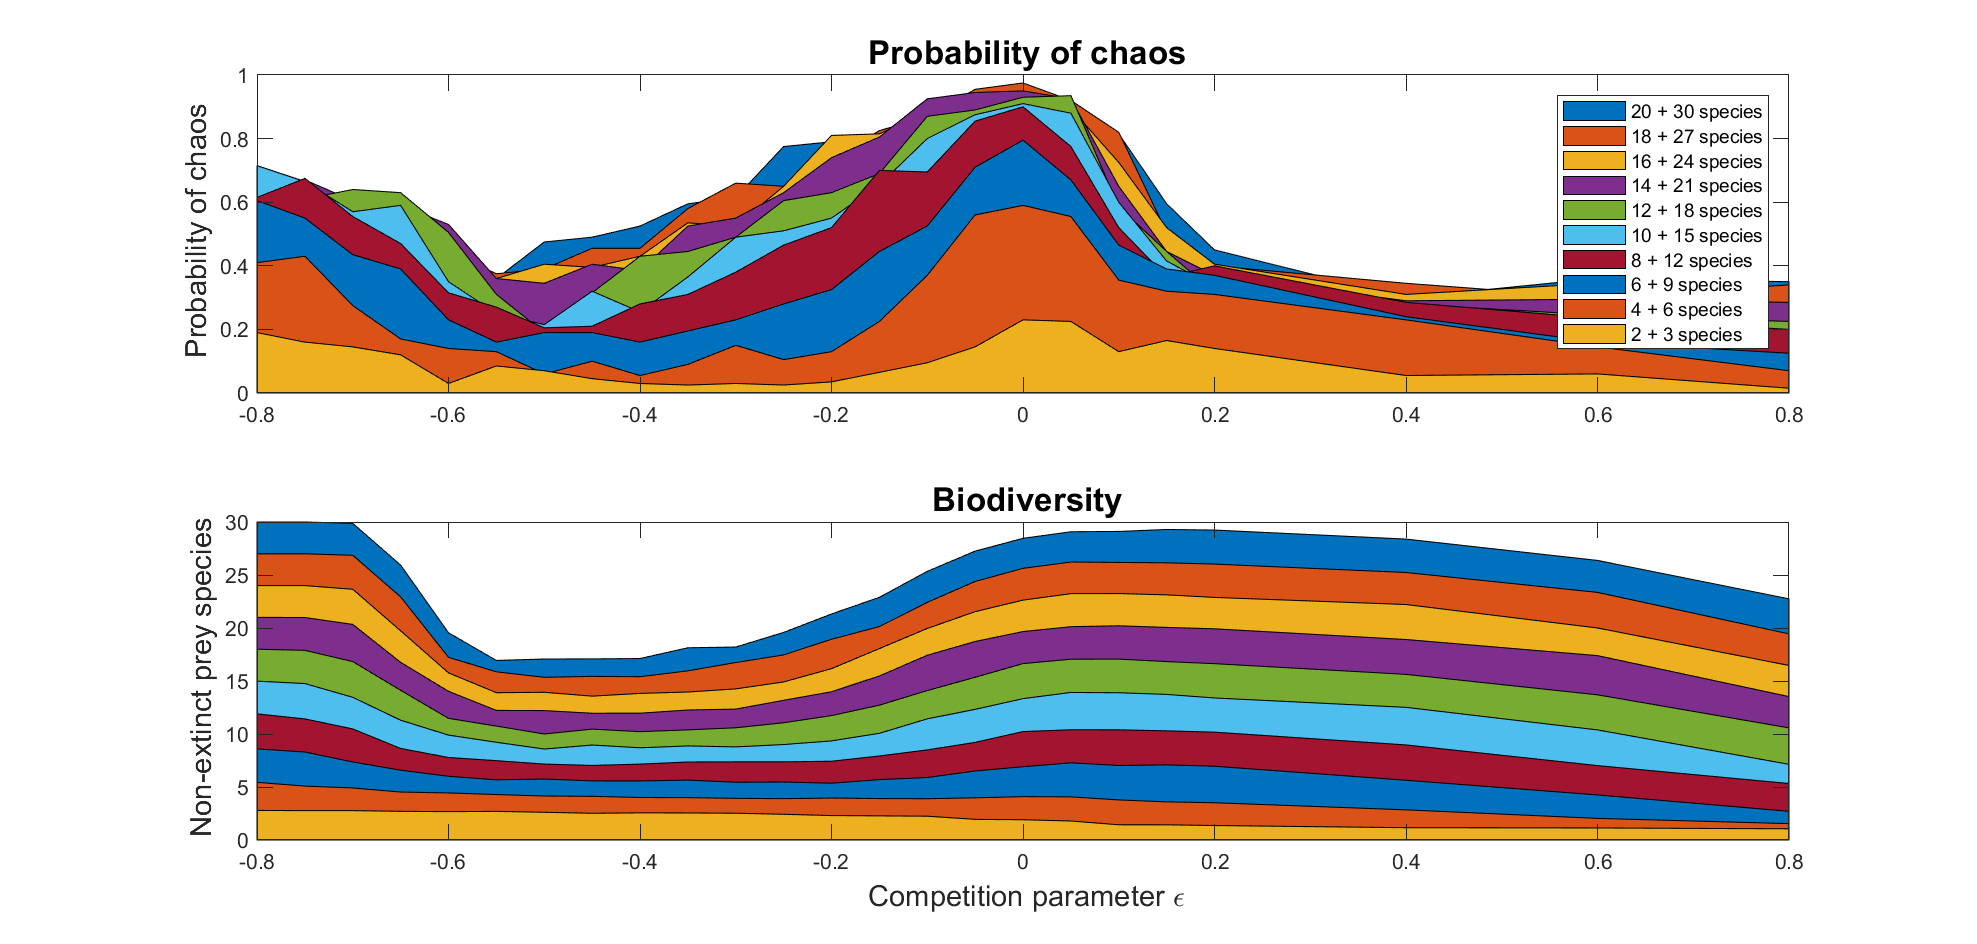
\includegraphics[width=1\columnwidth]{results_all.png}
	\end{center}
	\caption{Summary of the results of the whole set of simulations. The competition parameter $\epsilon$ is on the horizontal axis. The estimated probability of chaos is represented on the vertical one. Each panel corresponds to an ecosystem with a different number of interacting species. The exact number is shown in each box, as number of predators + number of prey.}
	\label{fig:AllProbabilities}
\end{figure}

\subsubsection{Biodiversity measurements}
\label{subsubsec:BiodiversityFigs}

For each simulation, a biodiversity index was estimated as the number of prey species whose population was higher than a minimum threshold of $\bioThreshold$ $mg$ $l^{-1}$, averaged respective to time.

\begin{figure}[H]
	\begin{center}
		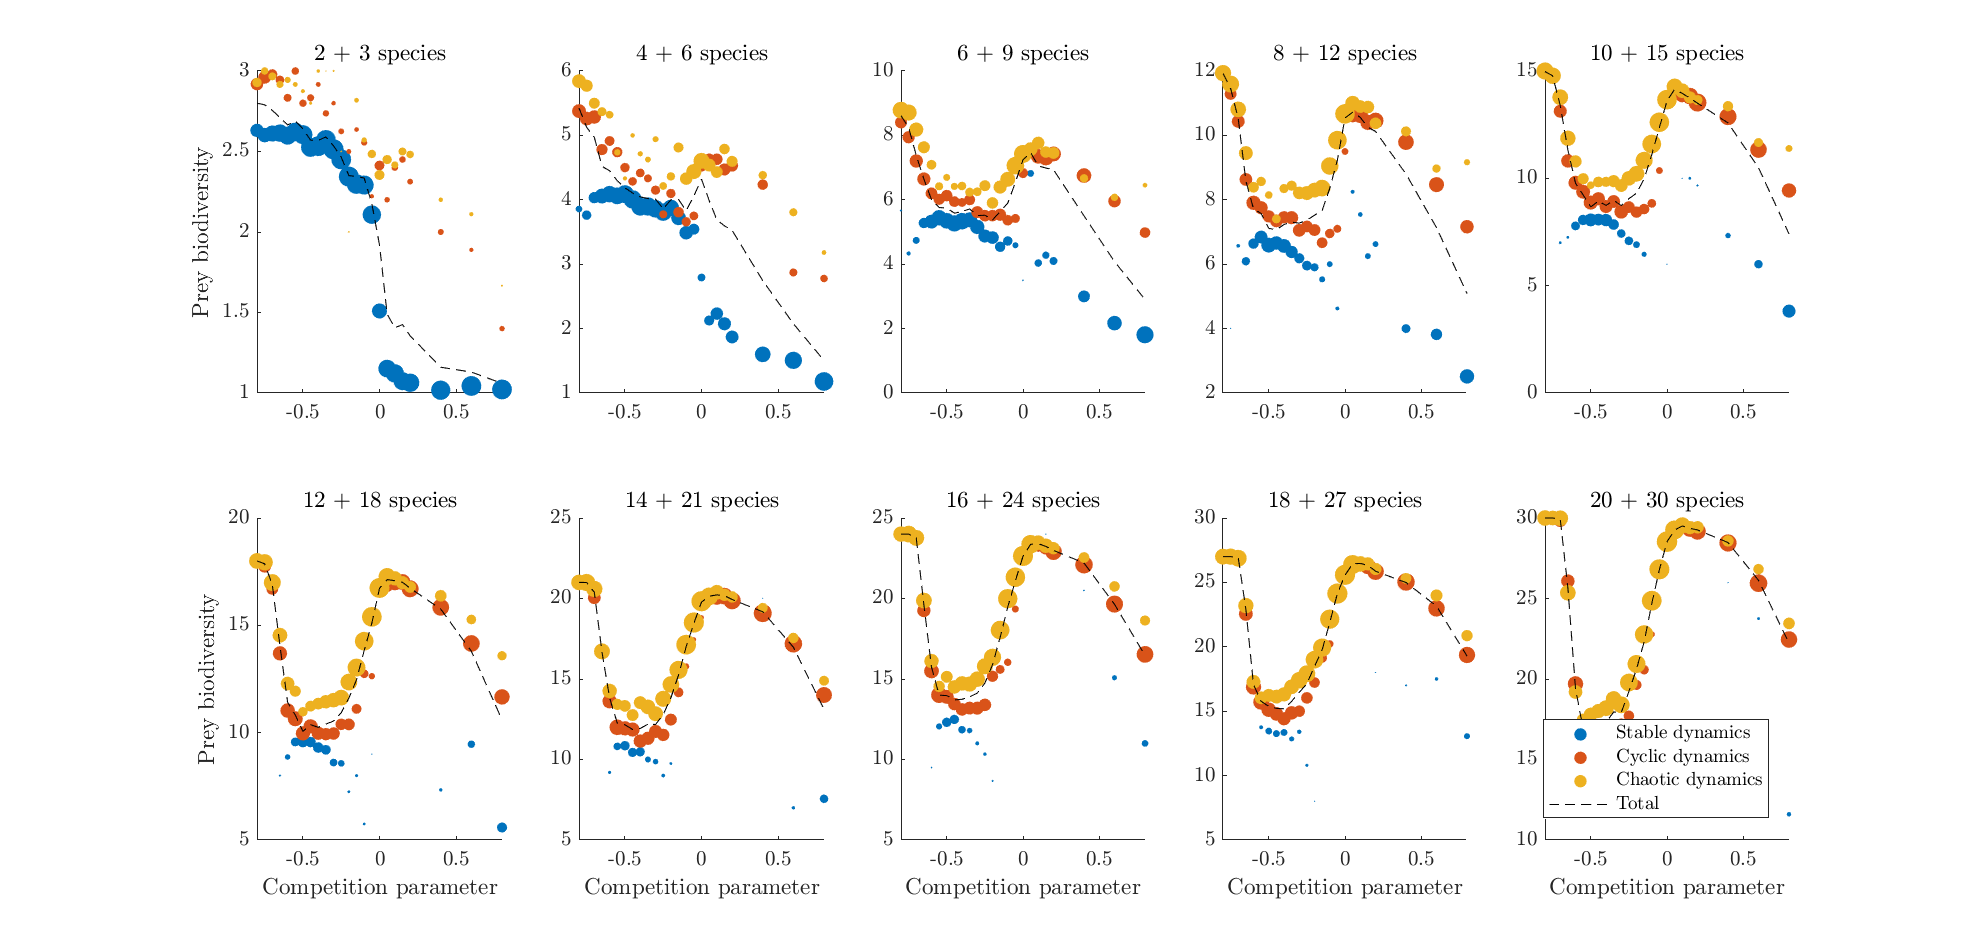
\includegraphics[width=1\columnwidth]{biod_split_by_dynamics.png}
	\end{center}
	\caption{Average prey biodiversity vs. competition parameter. Each panel shows a food network of a different size. For each value of the competition parameter, 200 randomly drawn ecosystems were simulated. The dashed line shows the average number of prey species of these 200 simulations. The white circles represent the average prey biodiversity of those simulations who had chaotic dynamics, the black circles represent the same for non-chaotic dynamics. The relative area of the white to the black circles represents the ratio of chaotic to regular dynamics.}
	\label{fig:BiodSplitByChaos}
\end{figure}

\begin{figure}[H]
	\begin{center}
		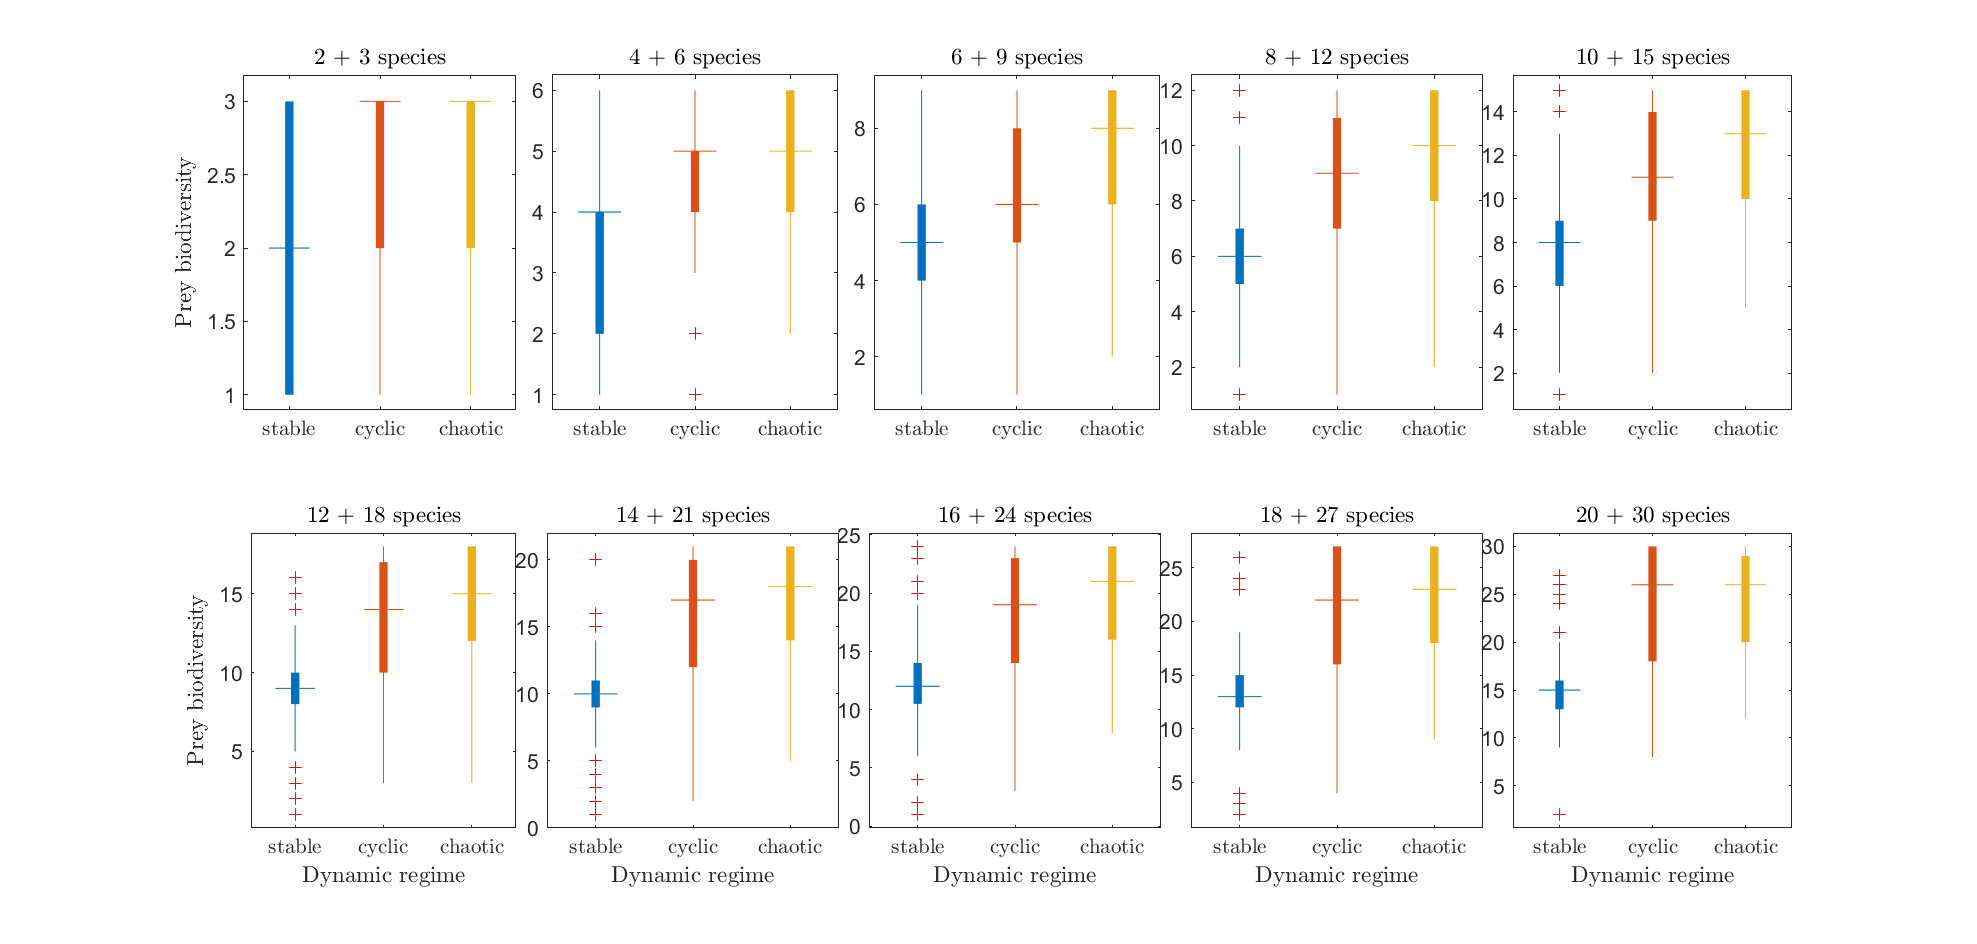
\includegraphics[width=1\columnwidth]{biod_box_and_whisker.png}
	\end{center}
	\caption{Box and whisker plot of the prey biodiversity, after being classified as regular or chaotic.}
	\label{fig:BiodBoxAndWhisker}
\end{figure}

\subsubsection{Flow chart}
\label{subsubsec:FlowChart}
In the spirit of reproducible research we made available all the analysis code used to draw our conclusions. Any interested researcher can clone it from a \textit{GitHub} repository \citep{Rodriguez-Sanchez-code-neuchaos} and, executing a single script, reproduce all our simulations and figures. This figure shows schematically what this script does:

\begin{figure}[H]
	\begin{center}
		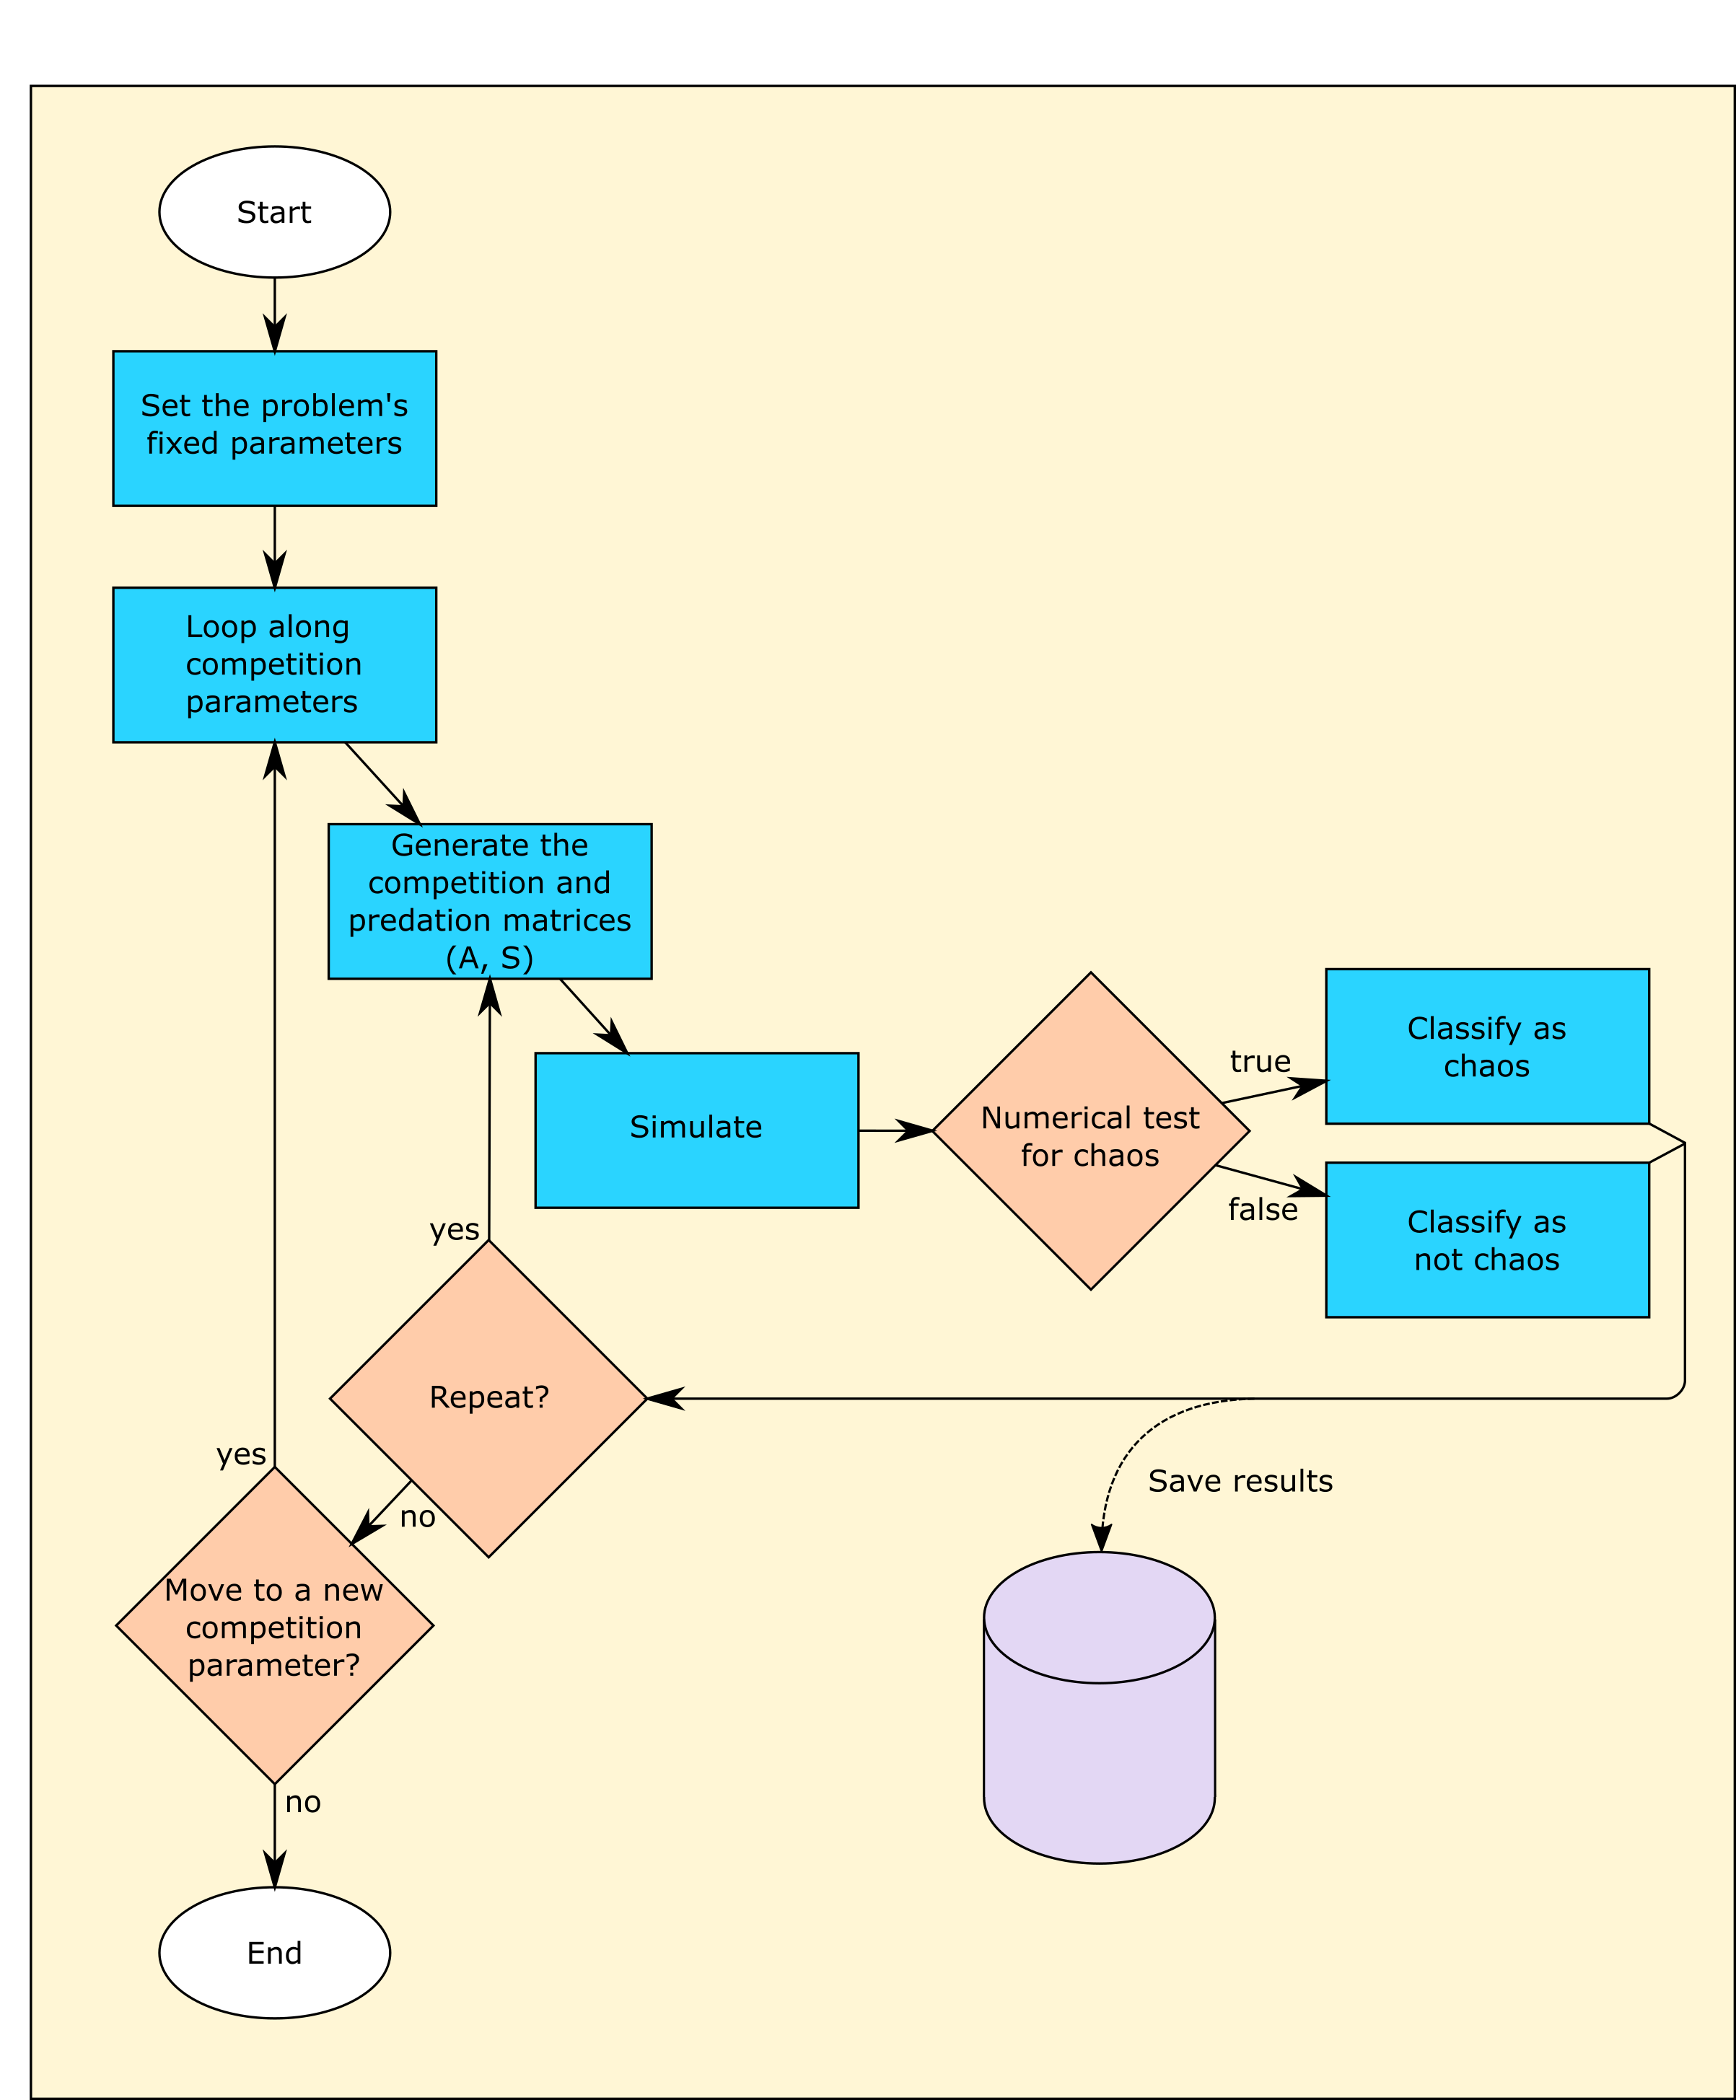
\includegraphics[width=0.8\columnwidth]{flow_chart.png}
	\end{center}
	\caption{Flow chart describing the numerical experiment. The source code is available at \textit{\texttt{https://doi.org/10.5281/zenodo.1319590}}.}
	\label{fig:FlowChart}
\end{figure}
